
%!TEX TS-program = xelatex
%!TEX encoding = UTF-8 Unicode

\documentclass[11pt,twoside,a4paper]{book}

	%Establecemos el tamaño de la hoja a a4 y el tamaño de los márgenes izquierdo y derecho al mínimo
	\usepackage[a4paper]{geometry} 

	% Paquetes para uso de matemáticas
	\usepackage{amssymb}

	% Para poder usar \boldsymbol que nos permite poner negrita a expresiones ``matemáticas'' en modo matemático.
	\usepackage{amsmath}

	% Paquete para introducir símbolos dingbats
	\usepackage{pifont}

	% Paquete para usar imágenes jpg y png
	\usepackage{graphicx}

	% Paquete para poder usar colores
	\usepackage{xcolor}
	
	% Paquete para soportar silabeo en castellano
	\usepackage[spanish]{babel}

	% Activate to begin paragraphs with an empty line rather than an indent
	\usepackage[parfill]{parskip}

	% Identar el comienzo de cada parrafo
	\usepackage{indentfirst}

	% Paquete para poder centrar verticalmente las columnas de las tablas
	\usepackage{array}
	
	% Permite usar enlaces (por ejemplo desde la tabla de contenidos)
	\usepackage{hyperref}
 
    \hypersetup{
        colorlinks,%
        citecolor=black,%
        filecolor=black,%
        linkcolor=black,%
        urlcolor=black
    }

	% Permite cambiar el títulos de las páginas
	\usepackage{fancyhdr}
	
	% Personalización de las cabeceras con fancyhdr
    \fancyhead{} % clear all header fields 
    \fancyfoot{} % clear all footer fields 
    \fancyhead[RE,LO]{\bfseries Compilación 1 }
    \fancyhead[RO,LE]{\small{\bfseries Jon Ander Hernández, Alberto Alonso y Gorka Blanco (JAG)}}
    \fancyfoot[LE,RO]{\thepage} 
    \fancyfoot[LO,CE]{} 
    \fancyfoot[CO,RE]{} 
    \renewcommand{\headrulewidth}{0.4pt} 
    \renewcommand{\footrulewidth}{0.4pt} 

    \pagestyle{fancy}

    \fancypagestyle{plain}{% 
    \fancyhead{} % clear all header fields 
    \fancyfoot{} % clear all footer fields 
    \fancyhead[RE,LO]{\bfseries Compilación 1 }
    \fancyhead[RO,LE]{\small{\bfseries Jon Ander Hernández, Alberto Alonso y Gorka Blanco (JAG)}}
    \fancyfoot[LE,RO]{\thepage} 
    \fancyfoot[LO,CE]{} 
    \fancyfoot[CO,RE]{} 
    \renewcommand{\headrulewidth}{0.4pt} 
    \renewcommand{\footrulewidth}{0.4pt}}


	% Podemos cambiar las fuentes por defecto Serif, San Serif, y Mono en _XeTeX_ y usar fuentes OpenType y AAT.
	\usepackage{fontspec,xltxtra,xunicode}
	\defaultfontfeatures{Mapping=tex-text}
	%\setromanfont[Mapping=tex-text]{Hoefler Text}
	%\setsansfont[Scale=MatchLowercase,Mapping=tex-text]{Gill Sans}
	%\setmonofont[Scale=MatchLowercase]{Andale Mono}

	% Paquete para poder incluir código fuente
	\usepackage{listings}

    % Establecemos los valores por defecto de Listings
	\lstset{
		language={C++},                              % Lenguaje por defecto
		%
		% estilos
		keywordstyle=\bfseries\ttfamily\color[rgb]{.8,.1,.2},	% estilos de palabras clave, identificadores, etc...
		identifierstyle=\ttfamily,
		commentstyle=\color[rgb]{0.1,0.5,0.1},			 
		stringstyle=\ttfamily\color[rgb]{0.2,0.2,.7},			
		basicstyle=\footnotesize,                    % the size of the fonts used for the code 
		%
		% numeración (desabilitadas en este momento :-)
		numbers=left,                                % where to put the line-numbers 
		numberstyle=\footnotesize,                   % size of the fonts used for the line-numbers 
		stepnumber=1,                                % the step between two line-numbers. 
		numbersep=5pt,                               % how far the line-numbers are from the code 
		%
		% espacios
		showspaces=false,                            % show spaces adding particular underscores 
		showstringspaces=false,                      % underline spaces within strings 
		showtabs=false, 							% show tabs within strings through particular underscores 
		tabsize=6,									% sets default tab-size to 2 spaces
		%
		% cuadro
		backgroundcolor=\color{white}, 				% sets background color (needs package) 
		frame=single, 								% adds a frame around the code
		rulecolor=\color[rgb]{.3,.3,.3},					% set the frame's color. 
		captionpos=b, 								% sets the caption-position to bottom 
		%
		% line breaking
		breaklines=true, 							% sets automatic line breaking 
		breakatwhitespace=false, 					% automatic breaks happen at whitespace 
		prebreak = \raisebox{0ex}[0ex][0ex]{\ensuremath{\hookleftarrow}} % Nos dibuja una flecha ``guay'' cuando el código no entra en una linea
	}

% Reescribimos algunas macros para cambiar algunos parámetros

	% Establecemos el interlineado a 1.2
	\renewcommand{\baselinestretch}{1.2}


\author{ \href{mailto:jahernandez002@ikasle.ehu.es}{Jon Ander Hernández} \and 
         \href{mailto:aalonso065@ikasle.ehu.es}{Alberto Alonso} \and
         \href{mailto:gblanco002@ikasle.ehu.es}{Gorka Blanco Gutierrez} \\[.5em] \and
         %
         \small\href{mailto:jahernandez002@ikasle.ehu.es}{jahernandez002@ikasle.ehu.es} \and 
         \small\href{mailto:aalonso065@ikasle.ehu.es}{aalonso065@ikasle.ehu.es} \and
         \small\href{mailto:gblanco002@ikasle.ehu.es}{gblanco002@ikasle.ehu.es} \\[1em] }
         
         
\title{%
	% Creamos un entorno de centrado
	\begin{centering}
		% Establecemos la fuente
		\fontspec[Ligatures={Common},Color=000000]{Hoefler Text}\fontsize{50pt}{50pt}\selectfont 
		% El título en grande
		Compilación I. 
	\end{centering}
	%
	\newline \Huge{1º Entrega}
	%
	% Dejamos un hueco flexible, de modo que los autores bajen hasta la parte de abajo del documento
	\vfill
}



\begin{document}

    % Para que fancyhdr no incluya un pie ni una cabecera en la portada
    \thispagestyle{empty}

    % Creamos la portada
    \maketitle

    \thispagestyle{empty}
    
    \cleardoublepage
    
    
    % Creamos la tabla de contenidos
    \tableofcontents

	
\part{Analizador léxico}


\chapter{Análisis léxico: Especificación de los tokens}
    
    \section{Espacios}
    
        \subsection{Descripción}
        
            Usamos este tipo de Token para representar el conjunto de espacios, aunque este Token será ignorado desde el nivel sintáctico.
        
            A la hora de interpretar el documento, emplearemos 2 autómatas. Uno para interpretar los espacios convencionales, y otro para interpretar los saltos de linea, ya que a medida que vamos leyendo el documento iremos contando el número linea para reportarlo en caso de error.
        
        \subsection{Atributos}
        
            Ninguno
            
	    \subsection{Espacios normales}
     
            \subsubsection{Expresión regular}
                \begin{lstlisting}[language=Perl]
[\ \t]+
                \end{lstlisting}

            \subsubsection{Autómata}
            
                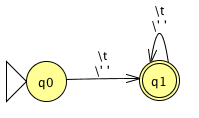
\includegraphics[scale=.7]{../Design/jflap/Espacio.png}
                
        \subsection{Saltos de linea}
        
            \subsubsection{Expresión regular}
            
                \begin{lstlisting}[language=Perl]
\n|\r|\r\n
                \end{lstlisting}
                
            \subsubsection{Autómata}
         
                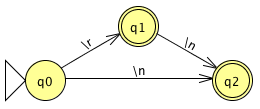
\includegraphics[scale=.7]{../Design/jflap/Salto_de_linea.png}
            
        \subsection{Notas}
        
            \begin{itemize}
            
                \item Con el método NextToken de la clase Tokenizer, podemos indicar si queremos filtrar los espacios y/o los saltos de linea.
            
            \end{itemize}
            
            \hfill
            \clearpage
            
            
            
    \section{Separadores}
    
        \subsection{Descripción}
        
            Usamos este tipo de Token para representar el conjunto de separadores :
            
            \begin{itemize}
                \item Paréntesis. Empleados para indicar los argumentos de los procedimientos.
                \item Punto y coma. Empleados para separar las instrucciones.
                \item Dos puntos. Para separar el tipo de los identificadores en las declaraciones de variables.
                \item Coma. Para separar los argumentos de los procedimientos, y los identificadores en las declaraciones de las variables.
            \end{itemize}
            
        \subsection{Expresión regular}
            
             \begin{lstlisting}[language=Perl]
[(),:;]
             \end{lstlisting}


        \subsection{Autómata}
            
	        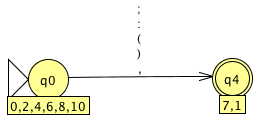
\includegraphics[scale=.7]{../Design/jflap/Separador.png}
	        
        \subsection{Atributos}
        
            \begin{itemize}
                \item Número de linea
                \item Número de columna
                \item Valor.
            \end{itemize}
            
            \hfill
            \clearpage
            
     
    
    \section{Comentario}
    
        \subsection{Descripción}
        
            Usamos este tipo de Token para representar los comentarios, aunque este Token será ignorado desde el nivel sintáctico.
            
            Los comentarios pueden ser multilinea, y aceptan cualquier contenido en su interior hasta encontrar el cierre del comentario.
        
        \subsection{Expresión regular}
            
             \begin{lstlisting}[language=Perl]
\/\*([^*]|(\*+[^*\/]))*\*+\/
             \end{lstlisting}
            
        \subsection{Autómata}
        
            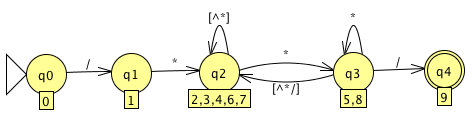
\includegraphics[scale=.7]{../Design/jflap/Comentario.png}

        \subsection{Atributos}
        
            \begin{itemize}
                \item Número de linea.
                \item Número de columna.
                \item Valor.
            \end{itemize}
            
            \hfill
            \clearpage
            


	\section{Identificador}

        \subsubsection{Descripción}
        
            Usamos este tipo de Token para representar un identificador.
            
            Los identificadores son de tipo Ada con subrayado: Empiezan por carácter alfabético, puede contener caracteres alfanuméricos o guión bajo, pero no puede comenzar ni terminar con un guión bajo ni puede contener dos guiones bajos seguidos.
            
        \subsection{Expresión regular}

            \begin{lstlisting}[language=Perl]
[a-zA-Z](_?[a-zA-Z0-9])*
            \end{lstlisting}

        \subsection{Autómata}
        
            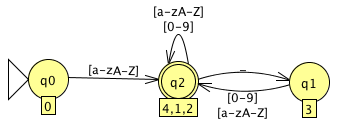
\includegraphics[scale=.7]{../Design/jflap/Identificador.png}

        \subsection{Atributos}
        
            \begin{itemize}
                \item Número de linea.
                \item Número de columna.
                \item Valor.
            \end{itemize}

            \hfill
            \clearpage
            



	\section{Constante entera}
    
        \subsection{Descripción}
        
            Usamos este tipo de Token para representar las constantes enteras.
        
        \subsection{Expresion regular}
        
            \begin{lstlisting}[language=Perl]
[0-9]+
            \end{lstlisting}

        \subsection{Autómata}
        
	        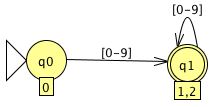
\includegraphics[scale=.7]{../Design/jflap/Constante_entera.png}

        \subsection{Atributos}
        
            \begin{itemize}
                \item Número de linea.
                \item Número de columna.
                \item Valor.
            \end{itemize}

            \hfill
            \clearpage
            
            
            
            
	\section{Constante real}

        \subsection{Descripción}

            Usamos este tipo de Token para representar las constantes reales, es decir números reales con decimales y exponencial.

        \subsection{Expresion regular}

            \begin{lstlisting}[language=Perl]
[0-9]+\.[0-9]+([eE][+\-]?[0-9]+)?
            \end{lstlisting}

        \subsection{Autómata}

            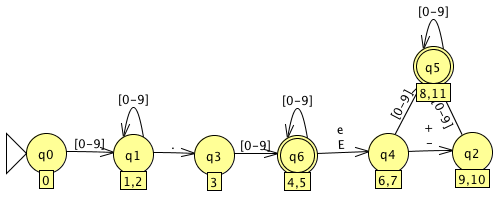
\includegraphics[scale=.7]{../Design/jflap/Constante_real.png}

        \subsection{Atributos}

            \begin{itemize}
                \item Número de linea.
                \item Número de columna.
                \item Valor.
            \end{itemize}

            \hfill
            \clearpage




	\section{Operadores}

        \subsection{Descripción}
        
            Usamos este tipo de Token para representar los operadores :
            
            \begin{itemize}
            
                \item Aritméticos
                \item Relacionales
                \item Operador asignación
                
            \end{itemize}
        
        \subsection{Operadores aritméticos}
        
            \begin{lstlisting}[language=Perl]
[+-*/]
            \end{lstlisting}

        \subsection{Operadores relacionales}

            \begin{lstlisting}[language=Perl]
[<>]|[/<>=]=
            \end{lstlisting}
            
        \subsection{Operador asignación}

            \begin{lstlisting}[language=Perl]
=
            \end{lstlisting}

        \subsection{Todos los operadores}

            \begin{lstlisting}[language=Perl]
[+-*/]|[<>]|[/<>=]=|=
            \end{lstlisting}

        \subsection{Autómata Operadores}

            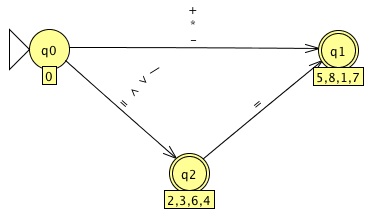
\includegraphics[scale=.7]{../Design/jflap/Operadores.png}

        \subsection{Atributos}

            \begin{itemize}
                \item Número de linea.
                \item Número de columna.
                \item Valor.
            \end{itemize}

            \hfill
            \clearpage



\section{Autómata competo unificado}

         \hspace{-7.8em}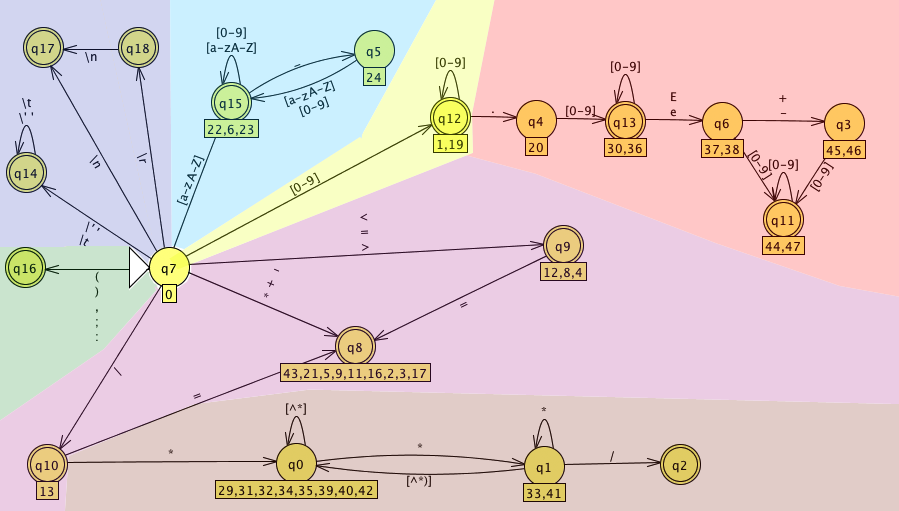
\includegraphics[scale=.61]{../Design/jflap/automata.png}

            \hfill
            \clearpage


 
\section{Listado de palabras reservadas}
    
        \subsection{Descripción}
        
        La palabras reservadas son identificadores reservados con un significado especial en nuestro lenguaje.
        
        \begin{itemize}
             \item programa
             \item procedimiento
             \item entrada
             \item salida
             \item si
             \item entonces
             \item fin
             \item hacer
             \item mientras
             \item salir
             \item get
             \item put\_line
       \end{itemize}

       \hfill
       \clearpage





	
\chapter{Casos de prueba. Entrada y salida obtenida}
	
	
\section{Programa lexicamente completo}
	
    \subsection{Programa}
	    
        \lstinputlisting{../ejemplos/ejem0.dat}
	
   \subsection{Salida}
	    
        \lstinputlisting[basicstyle=\small]{../ejemplos/ejem0_salida.txt}

    % Rellena el resto de la página, y termina la página actúal
    \hfill
    \clearpage

	

\section{Programa con comentarios erróneos}

    \subsection{Programa}
	    
        \lstinputlisting{../ejemplos/ejem1.dat}
	
   \subsection{Salida}
	    
        \lstinputlisting{../ejemplos/ejem1_salida.txt}

    % Rellena el resto de la página, y termina la página actúal
    \hfill
    \clearpage



\section{Programa con identificadores inválidos}

    \subsection{Programa}
	    
        \lstinputlisting{../ejemplos/ejem2.dat}
	
   \subsection{Salida}
	    
        \lstinputlisting{../ejemplos/ejem2_salida.txt}

    % Rellena el resto de la página, y termina la página actúal
    \hfill
    \clearpage




\section{Programa con constantes enteras erróneas}

    \subsection{Programa}
	    
        \lstinputlisting{../ejemplos/ejem3.dat}
	
   \subsection{Salida}
	    
        \lstinputlisting{../ejemplos/ejem3_salida.txt}

    % Rellena el resto de la página, y termina la página actúal
    \hfill
    \clearpage

	
	
\chapter{Mejoras}

\begin{itemize}

    \item Compilable en Windows, Mac OS X y Linux, mediante un Makefile generado con netbeans.

    \item Hemos implementado la práctica en C++ desde cero.
    
    \item La tabla de clases de caracteres incluye una columna Unknown que nos sirve para aceptar cualquier tipo de entrada en algunas transiciones. Como por ejemplo en los comentarios, que permite incluir cualquier carácter hasta llegar al final del comentario.
    
    \item Triggers. Los estados pueden contener una rutina que es ejecutada cuando se llega a dicho estado. Utilizamos esta funcionalidad en los comentarios para registrar los saltos de linea en los comentarios multilinea.
    
    \item La función NextToken del Tokenizer nos permite parametrizar si queremos filtrar los espacios y los saltos de linea.
    
    \item Leemos los ficheros mediante una abstracción que realiza buffering.
    
    \item Documentación escrita en \LaTeX.
    
\end{itemize}

	
	
\chapter{Horas invertidas}

    \section{Jon Ander Hernández}
    
        \begin{itemize}
            \item 1 hora en el estudio del enunciado.
            \item 2 horas en el estudio y diseño de los autómatas.
            \item 1 hora en la creación de los dibujos de los autómatas.
            \item 1 hora en el esqueleto de la documentación en \LaTeX.
            \item 4 horas de Extreme Programming (en Pair Programming) en la implementación.
         \end{itemize}
    
    \section{Alberto Alonso}
    
        \begin{itemize}
            \item 1 hora en estudio del enunciado y diseño de algoritmos.
            \item 30 minutos en los autómatas.
            \item 1 hora en el esqueleto de la aplicación.
            \item 15 minutos en la puesta a punto del subversion.
            \item 1 hora de implementación.
            \item 5 horas de Extreme Programming (en Pair Programming) en la implementación.
			\item 10 horas en la ETDS básica.
			\item 11 horas en la recopilación de información e implementación de la estructura base del analizador sintáctico/semántico.
			\item 9 horas en la programación de la información de tipos y la tabla de símbolos.
			\item 14 horas con la ETDS final.
			\item 8 horas con abstracciones funcionales, funciones de cadenas de texto y arreglos varios.
			\item 2.5 horas implementando el modo de pánico.
        \end{itemize}
    
    \section{Gorka Blanco Gutierrez}
    
        \begin{itemize}
            \item 1 hora en estudio del enunciado y diseño de algoritmos.
            \item 3 horas estudio y limpieza del antiguo código en C y Java.
            \item 1 hora de documentación en \LaTeX.
            \item 2 horas de Pair Programming.
        \end{itemize}
	
\end{document}  

